\documentclass{standalone}
\usepackage{tikz}
\usetikzlibrary{patterns, positioning}

\begin{document}
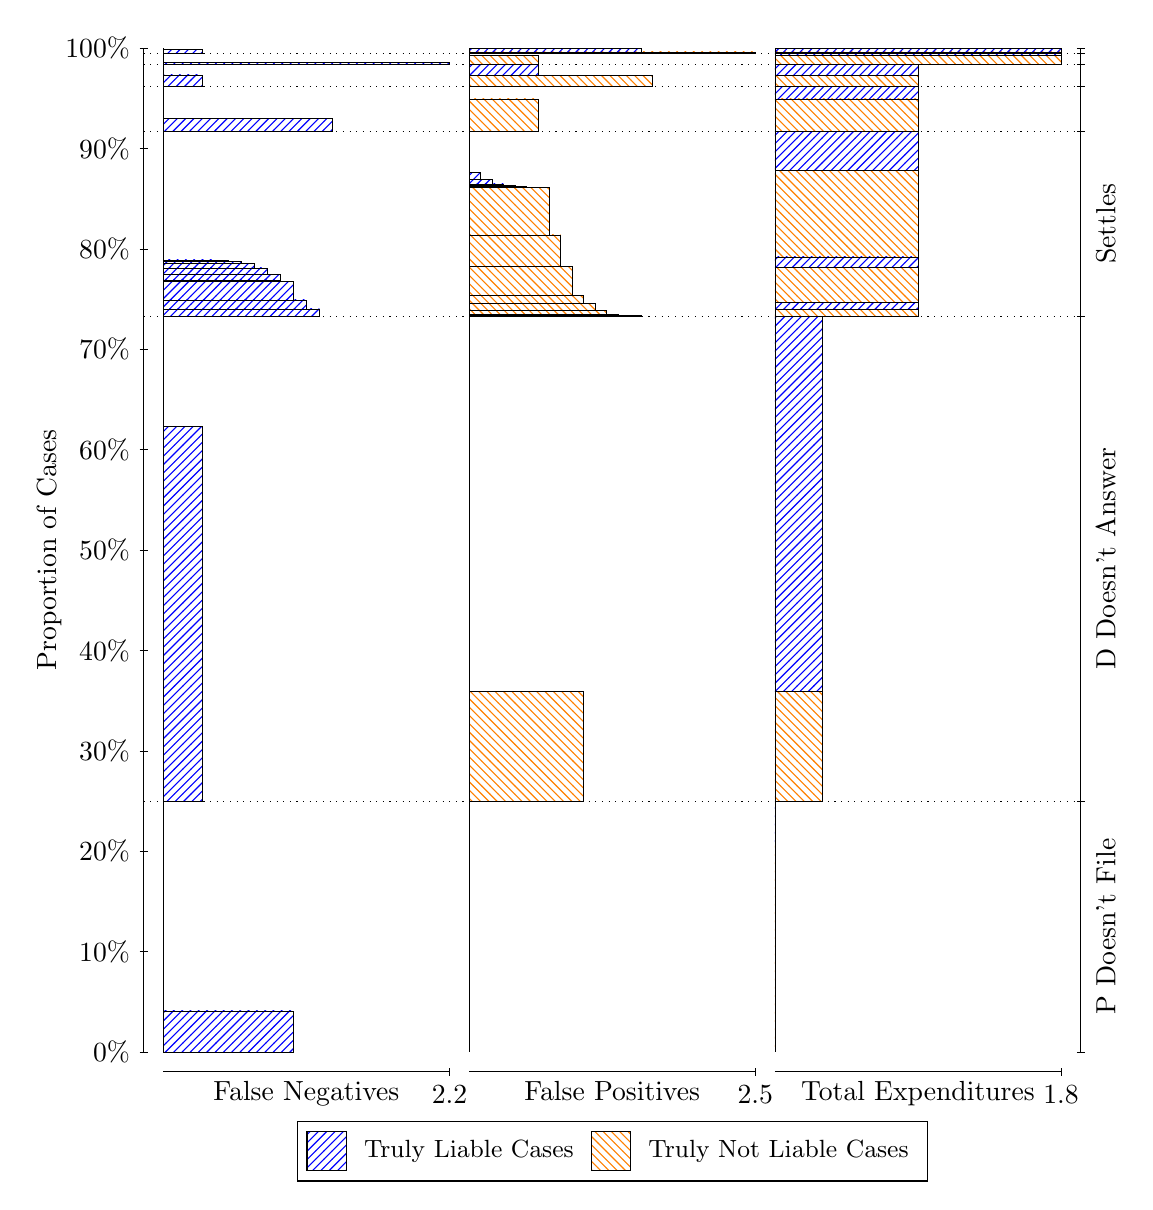
\begin{tikzpicture}
\draw[black, very thin] (1.5,1.75) -- (1.5,14.5);
\node[rotate=90, anchor=center] at (0.3, 8.125) {Proportion of Cases};
\draw[black, very thin] (1.45,1.75) -- (1.55,1.75);
\node[anchor=east] at (1.45, 1.75) {0\%};
\draw[black, very thin] (1.45,3.025) -- (1.55,3.025);
\node[anchor=east] at (1.45, 3.025) {10\%};
\draw[black, very thin] (1.45,4.3) -- (1.55,4.3);
\node[anchor=east] at (1.45, 4.3) {20\%};
\draw[black, very thin] (1.45,5.575) -- (1.55,5.575);
\node[anchor=east] at (1.45, 5.575) {30\%};
\draw[black, very thin] (1.45,6.85) -- (1.55,6.85);
\node[anchor=east] at (1.45, 6.85) {40\%};
\draw[black, very thin] (1.45,8.125) -- (1.55,8.125);
\node[anchor=east] at (1.45, 8.125) {50\%};
\draw[black, very thin] (1.45,9.4) -- (1.55,9.4);
\node[anchor=east] at (1.45, 9.4) {60\%};
\draw[black, very thin] (1.45,10.675) -- (1.55,10.675);
\node[anchor=east] at (1.45, 10.675) {70\%};
\draw[black, very thin] (1.45,11.95) -- (1.55,11.95);
\node[anchor=east] at (1.45, 11.95) {80\%};
\draw[black, very thin] (1.45,13.225) -- (1.55,13.225);
\node[anchor=east] at (1.45, 13.225) {90\%};
\draw[black, very thin] (1.45,14.5) -- (1.55,14.5);
\node[anchor=east] at (1.45, 14.5) {100\%};

\draw[black, very thin] (13.4,1.75) -- (13.4,14.5);
\draw[black, very thin] (13.35,1.75) -- (13.45,1.75);
\node[anchor=west] at (13.35, 1.75) {};
\draw[black, very thin] (13.35,4.936) -- (13.45,4.936);
\node[anchor=west] at (13.35, 4.936) {};
\draw[black, very thin] (13.35,11.095) -- (13.45,11.095);
\node[anchor=west] at (13.35, 11.095) {};
\draw[black, very thin] (13.35,13.445) -- (13.45,13.445);
\node[anchor=west] at (13.35, 13.445) {};
\draw[black, very thin] (13.35,14.017) -- (13.45,14.017);
\node[anchor=west] at (13.35, 14.017) {};
\draw[black, very thin] (13.35,14.294) -- (13.45,14.294);
\node[anchor=west] at (13.35, 14.294) {};
\draw[black, very thin] (13.35,14.429) -- (13.45,14.429);
\node[anchor=west] at (13.35, 14.429) {};
\draw[black, very thin] (13.35,14.5) -- (13.45,14.5);
\node[anchor=west] at (13.35, 14.5) {};

\draw[black, very thin, pattern color=blue, pattern=north east lines] (1.75,1.75) rectangle (3.4015,2.2713);
\draw[black, very thin, pattern color=orange, pattern=north west lines] (1.75,2.2713) rectangle (1.75,4.936);
\draw[black, very thin, pattern color=blue, pattern=north east lines] (1.75,4.936) rectangle (2.2455,9.6998);
\draw[black, very thin, pattern color=orange, pattern=north west lines] (1.75,9.6998) rectangle (1.75,11.095);
\draw[black, very thin, pattern color=blue, pattern=north east lines] (1.75,11.095) rectangle (3.7318,11.187);
\draw[black, very thin, pattern color=blue, pattern=north east lines] (1.75,11.187) rectangle (3.5667,11.3);
\draw[black, very thin, pattern color=blue, pattern=north east lines] (1.75,11.3) rectangle (3.4015,11.537);
\draw[black, very thin, pattern color=blue, pattern=north east lines] (1.75,11.537) rectangle (3.2364,11.556);
\draw[black, very thin, pattern color=blue, pattern=north east lines] (1.75,11.556) rectangle (3.2364,11.624);
\draw[black, very thin, pattern color=blue, pattern=north east lines] (1.75,11.624) rectangle (3.0712,11.707);
\draw[black, very thin, pattern color=blue, pattern=north east lines] (1.75,11.707) rectangle (2.9061,11.766);
\draw[black, very thin, pattern color=blue, pattern=north east lines] (1.75,11.766) rectangle (2.7409,11.788);
\draw[black, very thin, pattern color=blue, pattern=north east lines] (1.75,11.788) rectangle (2.5758,11.799);
\draw[black, very thin, pattern color=blue, pattern=north east lines] (1.75,11.799) rectangle (2.4106,11.81);
\draw[black, very thin, pattern color=orange, pattern=north west lines] (1.75,11.81) rectangle (1.75,13.445);
\draw[black, very thin, pattern color=blue, pattern=north east lines] (1.75,13.445) rectangle (3.897,13.608);
\draw[black, very thin, pattern color=orange, pattern=north west lines] (1.75,13.608) rectangle (1.75,14.017);
\draw[black, very thin, pattern color=blue, pattern=north east lines] (1.75,14.017) rectangle (2.2455,14.158);
\draw[black, very thin, pattern color=orange, pattern=north west lines] (1.75,14.158) rectangle (1.75,14.294);
\draw[black, very thin, pattern color=blue, pattern=north east lines] (1.75,14.294) rectangle (5.3833,14.316);
\draw[black, very thin, pattern color=orange, pattern=north west lines] (1.75,14.316) rectangle (1.75,14.429);
\draw[black, very thin, pattern color=blue, pattern=north east lines] (1.75,14.429) rectangle (2.2455,14.478);
\draw[black, very thin, pattern color=orange, pattern=north west lines] (1.75,14.478) rectangle (1.75,14.5);
\draw[black, very thin, pattern color=orange, pattern=north west lines] (5.6333,1.75) rectangle (5.6333,4.4147);
\draw[black, very thin, pattern color=blue, pattern=north east lines] (5.6333,4.4147) rectangle (5.6333,4.936);
\draw[black, very thin, pattern color=orange, pattern=north west lines] (5.6333,4.936) rectangle (7.0867,6.3311);
\draw[black, very thin, pattern color=blue, pattern=north east lines] (5.6333,6.3311) rectangle (5.6333,11.095);
\draw[black, very thin, pattern color=orange, pattern=north west lines] (5.6333,11.095) rectangle (7.8133,11.101);
\draw[black, very thin, pattern color=orange, pattern=north west lines] (5.6333,11.101) rectangle (7.668,11.107);
\draw[black, very thin, pattern color=orange, pattern=north west lines] (5.6333,11.107) rectangle (7.5227,11.12);
\draw[black, very thin, pattern color=orange, pattern=north west lines] (5.6333,11.12) rectangle (7.3773,11.167);
\draw[black, very thin, pattern color=orange, pattern=north west lines] (5.6333,11.167) rectangle (7.232,11.26);
\draw[black, very thin, pattern color=orange, pattern=north west lines] (5.6333,11.26) rectangle (7.0867,11.356);
\draw[black, very thin, pattern color=orange, pattern=north west lines] (5.6333,11.356) rectangle (6.9413,11.726);
\draw[black, very thin, pattern color=orange, pattern=north west lines] (5.6333,11.726) rectangle (6.796,12.128);
\draw[black, very thin, pattern color=orange, pattern=north west lines] (5.6333,12.128) rectangle (6.6507,12.73);
\draw[black, very thin, pattern color=blue, pattern=north east lines] (5.6333,12.73) rectangle (6.36,12.741);
\draw[black, very thin, pattern color=blue, pattern=north east lines] (5.6333,12.741) rectangle (6.2147,12.752);
\draw[black, very thin, pattern color=blue, pattern=north east lines] (5.6333,12.752) rectangle (6.0693,12.774);
\draw[black, very thin, pattern color=blue, pattern=north east lines] (5.6333,12.774) rectangle (5.924,12.833);
\draw[black, very thin, pattern color=blue, pattern=north east lines] (5.6333,12.833) rectangle (5.7787,12.916);
\draw[black, very thin, pattern color=blue, pattern=north east lines] (5.6333,12.916) rectangle (5.6333,13.445);
\draw[black, very thin, pattern color=orange, pattern=north west lines] (5.6333,13.445) rectangle (6.5053,13.854);
\draw[black, very thin, pattern color=blue, pattern=north east lines] (5.6333,13.854) rectangle (5.6333,14.017);
\draw[black, very thin, pattern color=orange, pattern=north west lines] (5.6333,14.017) rectangle (7.9587,14.154);
\draw[black, very thin, pattern color=blue, pattern=north east lines] (5.6333,14.154) rectangle (6.5053,14.294);
\draw[black, very thin, pattern color=orange, pattern=north west lines] (5.6333,14.294) rectangle (6.5053,14.407);
\draw[black, very thin, pattern color=blue, pattern=north east lines] (5.6333,14.407) rectangle (5.6333,14.429);
\draw[black, very thin, pattern color=orange, pattern=north west lines] (5.6333,14.429) rectangle (9.2667,14.451);
\draw[black, very thin, pattern color=blue, pattern=north east lines] (5.6333,14.451) rectangle (7.8133,14.5);
\draw[black, very thin, pattern color=orange, pattern=north west lines] (9.5167,1.75) rectangle (9.5167,4.4147);
\draw[black, very thin, pattern color=blue, pattern=north east lines] (9.5167,4.4147) rectangle (9.5167,4.936);
\draw[black, very thin, pattern color=orange, pattern=north west lines] (9.5167,4.936) rectangle (10.122,6.3311);
\draw[black, very thin, pattern color=blue, pattern=north east lines] (9.5167,6.3311) rectangle (10.122,11.095);
\draw[black, very thin, pattern color=orange, pattern=north west lines] (9.5167,11.095) rectangle (11.333,11.188);
\draw[black, very thin, pattern color=blue, pattern=north east lines] (9.5167,11.188) rectangle (11.333,11.271);
\draw[black, very thin, pattern color=orange, pattern=north west lines] (9.5167,11.271) rectangle (11.333,11.717);
\draw[black, very thin, pattern color=blue, pattern=north east lines] (9.5167,11.717) rectangle (11.333,11.848);
\draw[black, very thin, pattern color=orange, pattern=north west lines] (9.5167,11.848) rectangle (11.333,12.944);
\draw[black, very thin, pattern color=blue, pattern=north east lines] (9.5167,12.944) rectangle (11.333,13.445);
\draw[black, very thin, pattern color=orange, pattern=north west lines] (9.5167,13.445) rectangle (11.333,13.854);
\draw[black, very thin, pattern color=blue, pattern=north east lines] (9.5167,13.854) rectangle (11.333,14.017);
\draw[black, very thin, pattern color=orange, pattern=north west lines] (9.5167,14.017) rectangle (11.333,14.154);
\draw[black, very thin, pattern color=blue, pattern=north east lines] (9.5167,14.154) rectangle (11.333,14.294);
\draw[black, very thin, pattern color=orange, pattern=north west lines] (9.5167,14.294) rectangle (13.15,14.407);
\draw[black, very thin, pattern color=blue, pattern=north east lines] (9.5167,14.407) rectangle (13.15,14.429);
\draw[black, very thin, pattern color=orange, pattern=north west lines] (9.5167,14.429) rectangle (13.15,14.451);
\draw[black, very thin, pattern color=blue, pattern=north east lines] (9.5167,14.451) rectangle (13.15,14.5);
\draw[black, dotted] (1.5,4.936) -- (13.4,4.936);
\draw[black, dotted] (1.5,11.095) -- (13.4,11.095);
\draw[black, dotted] (1.5,13.445) -- (13.4,13.445);
\draw[black, dotted] (1.5,14.017) -- (13.4,14.017);
\draw[black, dotted] (1.5,14.294) -- (13.4,14.294);
\draw[black, dotted] (1.5,14.429) -- (13.4,14.429);
\draw[black, very thin] (1.75,1.5) -- (5.3833,1.5);
\node[anchor=north] at (3.5667, 1.5) {False Negatives};
\draw[black, very thin] (5.3833,1.45) -- (5.3833,1.55);
\node[anchor=north] at (5.3833, 1.45) {2.2};

\draw[black, very thin] (5.6333,1.5) -- (9.2667,1.5);
\node[anchor=north] at (7.45, 1.5) {False Positives};
\draw[black, very thin] (9.2667,1.45) -- (9.2667,1.55);
\node[anchor=north] at (9.2667, 1.45) {2.5};

\draw[black, very thin] (9.5167,1.5) -- (13.15,1.5);
\node[anchor=north] at (11.333, 1.5) {Total Expenditures};
\draw[black, very thin] (13.15,1.45) -- (13.15,1.55);
\node[anchor=north] at (13.15, 1.45) {1.8};

\node[black, centered, rotate=90] at (13.72, 3.343) {P Doesn't File};
\node[black, centered, rotate=90] at (13.72, 8.0154) {D Doesn't Answer};
\node[black, centered, rotate=90] at (13.72, 12.27) {Settles};





\draw (7.449999999999999,1.5) node[draw=none] (baseCoordinate) {};
\begin{scope}[align=center]
        \matrix[scale=0.5, draw=black, below=0.5cm of baseCoordinate, nodes={draw}, column sep=0.1cm]{
            \node[rectangle, draw, minimum width=0.5cm, minimum height=0.5cm, pattern=north east lines, pattern color=blue] {}; &
            \node[draw=none, font=\small] (B) {Truly Liable Cases}; &
            \node[rectangle, draw, minimum width=0.5cm, minimum height=0.5cm, pattern=north west lines, pattern color=orange] {}; &
            \node[draw=none, font=\small] (B) {Truly Not Liable Cases}; \\
            };
\end{scope}

\end{tikzpicture}
\end{document}